\section*{Exercises}
\addcontentsline{toc}{section}{Exercises}

\begin{excersizelist}

% \item As seen in \eqref{eq:utimprespstep} and Figure~\zref{fig:rectpulsedelta} the impulse response of the integrator $I_\infty$ is the step function $u(t)$.  Is the mode of convergence for the limit in~\eqref{eq:utimprespstep} pointwise?  Is it uniform? (see Section~\zref{sec:convergence-signals} for definitions of these modes of convergence).
% \begin{solution}
% The convergence is pointwise.  If $t \leq 0$ then $I_\infty(p_\gamma,t) = 0 = u(t)$ so only remains to consider what happens for $t > 0$.  Fix $t > 0$ and for any $\epsilon > 0$ we can choose $\gamma$ large enough that $I_\infty(p_\gamma,t) = 1$
% \end{solution}

% \item \label{excer:distributivecommutive} Show that convolution distributes with addition and commutes with scalar multiplication, that is, show that $a(x*w) + b(y*w) = (ax+by)*w$.
% \begin{solution}
% \begin{align*}
% a (x * w) + b (y * w) &= a \int_{-\infty}^{\infty} x(\tau) w(t - \tau) d\tau + b \int_{-\infty}^{\infty} y(\tau) w(t - \tau) d\tau \\
% &= \int_{-\infty}^{\infty} \big(ax(\tau) + by(\tau)\big) w(t - \tau) d\tau\\
% &= (ax + by) * w.
% \end{align*}
% \end{solution}

% \item \label{excer:convassociative} Show that convolution is associative.  That is, if $x,y,z$ are signals then $x*(y*z) = (x*y)*z$. 
% \begin{solution}
% \begin{align*}
% (x*y)*z &= \int_{-\infty}^\infty (x*y)(\tau) z(t - \tau) d\tau \\
% &= \int_{-\infty}^\infty \int_{-\infty}^\infty x(\kappa) y(\tau-\kappa) z(t - \tau) d\kappa d\tau \\
% &= \int_{-\infty}^\infty x(\kappa)  \int_{-\infty}^\infty y(\tau-\kappa) z(t - \tau)  d\tau d\kappa  \qquad \text{(swap order of integration)} \\
% &= \int_{-\infty}^\infty x(\kappa)  \int_{-\infty}^\infty y(\nu) z(t - \kappa - \nu)  d\tau d\kappa  \qquad \text{(change variable $\nu = \tau-\kappa$)} \\
% &= \int_{-\infty}^\infty x(\kappa)  (y * z)(t - \kappa) d\kappa \\
% &= x*(y*z).
% \end{align*}
% The exchange of integration order can be justified using Fubini's theorem whenever the all of the convolutions involved in $x*(y*z) = (x*y)*z$ exist.
% \end{solution}

\item State whether each of the following systems are: causal, linear, shift-invariant, or stable.  Plot the impulse and step response of the systems whenever they exist.  In each case, assume the domain to be the set of locally integrable signals.
\begin{enumerate}
\item $Hx(t) = 3x(t - 1) - 2x(t+1)$
\item $Hx(t) = \sin\big(2\pi x(t)\big)$
\item $Hx(t) = t^2 x(t)$
\item $Hx(t) = \int_{-1/2}^{1/2} \cos(\pi\tau) x(t + \tau) d\tau$
\end{enumerate}

\begin{solution}

(a) The system can be written as $H(x) = 3T_{1}(x) - 2T_{-1}(x)$ which is a linear combination of shifters.  Since the shifter is linear and shift-invariant $H$ will be also (Section~\zref{sec:line-comb-comp} of the notes).  Linearity can also be shown directly
\begin{align*}
H(ax + by)  &= 3\big( a x(t-1) + by(t-1) \big)  - 2\big( a x(t+1) + by(t+1) \big) \\
&= a\big(3x(t-1)-2x(t+1)\big) + b\big(3y(t-1)-2y(t+1)\big) \\
&= aHx + bHy.
\end{align*}
Shift-invariance can also be shown directly
\begin{align*}
T_\tau Hx(t) &= H x(t-\tau) \\
&= 3x(t-1-\tau)  - 2x(t+1-\tau) \\
&= 3T_\tau x(t-1)  - 2T_\tau x(t+1) \\
&= HT_\tau x(t).
\end{align*}
The system is stable because for every input signal bounded less than $M > 0$, that is, for all input signals $x$ such that $\abs{x(t)} < M$ for all $t \in \reals$, we can choose $K = 5M$ and
\[
\sabs{Hx(t)} = \sabs{3x(t-1-\tau)  - 2x(t+1-\tau)} \leq 3\abs{x(t-1-\tau)} + 2\abs{x(t+1-\tau)}  < 5M = K,
\]
i.e., the output signal is bounded less than $K$.  The system is not causal, because it depends on the input signal $x$ at time $t+1$, i.e., in the `future'.  The system is not regular because it  is a linear combination of time shifters, and these are not regular, they don't formally have an impulse response (Section~\zref{sec:conv-regul-syst} of the notes).  The system does have a step response equal to $H(u,t) = 3u(t-1)  - 2u(t+1)$ that is plotted in the figures below.

(b) The system is causal, in fact, it is memoryless since it only depends on the input signal $x$ at time $t$, i.e. the `present' time.  The system $Hx(t) = \sin\big(2\pi x(t)\big)$ is shift-invariant because 
 \[
 H T_\tau x(t) = \sin\big(2\pi T_\tau x(t)\big) = \sin\big(2\pi x(t-\tau)\big) = T_\tau H x(t).
 \]
 The system is not linear since $H(ax,t) = \sin\big(2\pi a x(t)\big) \neq a \sin\big(2\pi x(t)\big)$ in general.  The system is stable, for every input signal $x$ with absolute value bounded below $M$ we have
\[
\abs{\sin(x(t))} = \abs{\frac{e^{jx(t)} - e^{-jx(t)}}{2j}} \leq \frac{\abs{e^{jx(t)}} + \abs{e^{-jx(t)}}}{2} < e^M
\] 
and so, choosing $K = e^{M}$ we find that $\abs{Hx(t)} < K$.  Because the system is not linear, it is not regular. It does have a step response equal to $Hu(t) = \sin\big(2\pi u(t)\big) = 0$.  Also acceptable is that is doesn't have a step response because this is a feature we developed for linear shift-invariant systems.

(c) The system is causal and also memoryless.  The system $Hx(t) = t^2x(t)$ is linear because 
\[
H(ax+by) = t^2(ax+by) = at^2x + bt^2y = aH x + bHy.
\]
The system is not shift-invariant because
\[
T_\tau H x(t) = (t-\tau)^2x(t-\tau) \neq H T_\tau x(t) = t^2 x(t - \tau)
\]
in general.  The system is not regular because it is not shift-invariant.  The system does not have an impulse response.  It does have a step response equal to $Hu(t) = t^2u(t)$.  This is plotted in the figures below.  Also acceptable is that is doesn't have a step response because this is a feature we developed for linear shift-invariant systems.  The system is not stable, for example the input step $u$ is bounded below $M > 1$ but the output $Hu$ is not bounded, it grows indefinitely as $t \to \infty$.

(d) Put $h(t) = \cos(\pi t) \rect(t)$ where $h$ is the rectangle function (see~(\zref{eq:rectfuncdefn}) of the lecture notes).  Now
\begin{align*}
Hx(t) &= \int_{-1/2}^{1/2} \cos(\pi\tau) x(t + \tau) d\tau \\
&=\int_{-1/2}^{1/2} \cos(-\pi\tau) x(t - \tau) d\tau & \text{(change var $\tau=-\tau$)}\\
&=\int_{-\infty}^{\infty} \cos(-\pi\tau)\rect(t) x(t - \tau) d\tau \\
&=\int_{-\infty}^{\infty} h(\tau) x(t - \tau) d\tau \\
&= (h*x)(t).
\end{align*}
Thus, $H$ is the regular system with impulse response $h(t) = \cos(\pi t) \rect(t)$.  A plot of $h$ is given below.  Since $H$ is regular it is also linear and shift-invariant.  The impulse response $h$ is absolutely  integrable with $\|h\|_1 = \tfrac{2}{\pi}$ and so $H$ is stable.  The system $H$ is not causal because $h$ is nonzero with some $t < 0$, specifically those $t \in (-\tfrac{1}{2},\tfrac{1}{2})$.  The step response is given by applying the integrator system $I_\infty$ to $h$, that is, 
\begin{align*}
I_\infty h(t) = \int_{-\infty}^t h(\tau) d\tau = \begin{cases}
0 & t \leq -\tfrac{1}{2} \\
\int_{-1/2}^t \cos(\pi\tau) d\tau = \big(\sin(\pi t) + 1\big)/\pi & -\tfrac{1}{2} < t \leq \tfrac{1}{2} \\
\tfrac{2}{\pi} & t > \tfrac{1}{2}.
\end{cases}
\end{align*}

\begin{center}
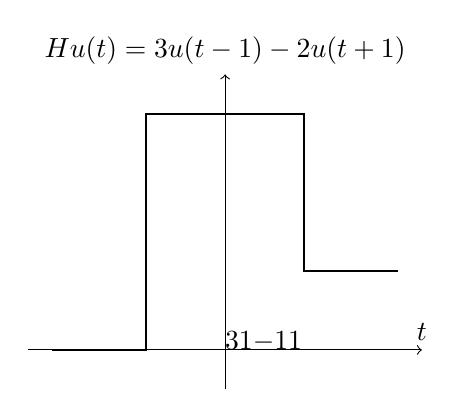
\begin{tikzpicture}
    %\draw[very thin,color=gray] (-0.1,-1.1) grid (3.9,3.9);
    \draw[->] (-2.5,0) -- (2.5,0) node[above] {$t$};
    \draw[->] (0,-0.5) -- (0,3.5) node[above] {$H u(t) = 3u(t-1)  - 2u(t+1)$};
    %\draw[color=black] plot[id=x] function{1/x^2} 
    %    node[right] {$f(t) = t^{-2}$};
    \draw[thick] (-2.2,0)--(-1,0)--(-1,3)--(1,3)--(1,1)--(2.2,1);
    \htick{3} node[pos=0.5,above left] {$3$};
    \htick{1} node[pos=0.5,left] {$1$};
    \vtick{-1} node[pos=0.5,below] {$-1$};
    \vtick{1} node[pos=0.5,below] {$1$};
    %\draw[color=black] plot[id=exp] function{0.05*exp(x)} 
    %    node[right] {$f(t) = \frac{1}{20} e^t$};
\end{tikzpicture} \;\;
\begin{tikzpicture}
    %\draw[very thin,color=gray] (-0.1,-1.1) grid (3.9,3.9);
    \draw[->] (-2.5,0) -- (2.5,0) node[above] {$t$};
    \draw[->] (0,-0.5) -- (0,3.5) node[above] {$Hu(t) = t^2u(t)$};
    %\draw[color=black] plot[id=x] function{1/x^2} 
    %    node[right] {$f(t) = t^{-2}$};
    \draw[thick] (-2.2,0)--(0,0);
    \draw[color=black,thick,domain=0:2.2,samples=50] plot[id=x] function{x*x*3/5};
    \htick{3*3/5} node[pos=0.5,above left] {$3$};
    \htick{3/5} node[pos=0.5,left] {$1$};
    \vtick{-1} node[pos=0.5,below] {$-1$};
    \vtick{1} node[pos=0.5,below] {$1$};
    %\draw[color=black] plot[id=exp] function{0.05*exp(x)} 
    %    node[right] {$f(t) = \frac{1}{20} e^t$};
\end{tikzpicture} 
\\ \vspace{0.2cm}
\begin{tikzpicture}
\begin{scope}[xscale=2,yscale=2.5]
    %\draw[very thin,color=gray] (-0.1,-1.1) grid (3.9,3.9);
    \draw[->] (-1.5,0) -- (1.5,0) node[above] {$t$};
    \draw[->] (0,-0.25) -- (0,1.25) node[above] {$h(t) = \cos(\pi t) \rect(t)$};
    %\draw[color=black] plot[id=x] function{1/x^2} 
    %    node[right] {$f(t) = t^{-2}$};
    \draw[thick] (-1.3,0)--(-1/2,0);
    \draw[thick] (1.3,0)--(1/2,0);
    \draw[color=black,thick,domain=-0.5:0.5,samples=50] plot[id=x] function{cos(pi*x)};
    %\draw[color=black] plot[id=exp] function{0.05*exp(x)} 
    %    node[right] {$f(t) = \frac{1}{20} e^t$};
\end{scope}
\begin{scope}[yscale=2.5]
    \htick{1} node[pos=0.5,above left] {$1$};
\end{scope}
\begin{scope}[xscale=2]
    \vtick{-1/2} node[pos=0.5,below] {$-\tfrac{1}{2}$};
    \vtick{1/2} node[pos=0.5,below] {$\tfrac{1}{2}$};
\end{scope}
\end{tikzpicture} \;\;
\begin{tikzpicture}
\begin{scope}[xscale=2,yscale=2.5]
    %\draw[very thin,color=gray] (-0.1,-1.1) grid (3.9,3.9);
    \draw[->] (-1.5,0) -- (1.5,0) node[above] {$t$};
    \draw[->] (0,-0.25) -- (0,1.25) node[above] {$I_\infty h(t)$};
    %\draw[color=black] plot[id=x] function{1/x^2} 
    %    node[right] {$f(t) = t^{-2}$};
    \draw[thick] (-1.3,0)--(-1/2,0);
    \draw[thick] (1.3,2/pi)--(1/2,2/pi);
    \draw[color=black,thick,domain=-0.5:0.5,samples=50] plot[id=x] function{(sin(pi*x)+1)/pi};
    %\draw[color=black] plot[id=exp] function{0.05*exp(x)} 
    %    node[right] {$f(t) = \frac{1}{20} e^t$};
\end{scope}
\begin{scope}[yscale=2.5]
    \htick{1} node[pos=0.5,above left] {$1$};
\end{scope}
\begin{scope}[xscale=2]
    \vtick{-1/2} node[pos=0.5,below] {$-\tfrac{1}{2}$};
    \vtick{1/2} node[pos=0.5,below] {$\tfrac{1}{2}$};
\end{scope}
\end{tikzpicture} 
\end{center}

\end{solution}


\item Show that the system $Hx(t) = \int_{-1}^{1} \sin(\pi\tau) x(t + \tau) d\tau$ is linear shift-invariant and regular.  Find and sketch the impulse response and the step response.
\begin{solution}
The easy way is to spot the impulse response directly.  Observe that
\begin{align*}
H(x)(t) &= \int_{-1}^{1} \sin(\pi\tau) x(t + \tau) d\tau \\
&= \int_{-\infty}^\infty \rect(\tau/2) \sin(\pi\tau) x(t + \tau) d\tau\\
&= -\int_{\infty}^{-\infty} \rect(-\tau/2) \sin(-\pi\tau) x(t - \tau) d\tau \qquad \text{(ch. var. $\tau \to -\tau$)} \\
&= -\int_{-\infty}^{\infty} \rect(\tau/2) \sin(\pi\tau) x(t - \tau) d\tau \\
&= (h * x)(t),
\end{align*}
where we put $h(t) = -\rect(t/2) \sin(\pi t)$.  It follows that $h$ is the impulse response of $H$.  Since $h$ has an impulse resposne it is regular, and since it is regular its also linear and time invariant.

The hard way is to first show linear, then show time invariance, and then find this impulse response as the limit 
\[
h = \lim_{\gamma \rightarrow \infty} H p_\gamma.
\]
where the function 
\[
p_\gamma(t) = \begin{cases}
\gamma, & 0 < t \leq \frac{1}{\gamma} \\
0, & \text{otherwise},
\end{cases}
\]
is introduced in Section~\zref{sec:conv-regul-syst}.  We have
\begin{align*}
H(ax+by) &= \int_{-1}^{1} \sin(\pi\tau) \big( ax(t + \tau) + by(t + \tau) \big) d\tau \\
&= a \int_{-1}^{1} \sin(\pi\tau) x(t + \tau) d\tau + b\int_{-1}^{1} \sin(\pi\tau)  y(t + \tau) \big) d\tau \\
&= aH(x) + bH(y),
\end{align*}
and so, $H$ is linear.  We also have
\begin{align*}
H\big(T_k(x)\big) &= \int_{-1}^{1} \sin(\pi\tau) T_k(x)(t + \tau) d\tau \\
&= \int_{-1}^{1} \sin(\pi\tau) x(t + \tau - k) d\tau \\
&= T_k \left( \int_{-1}^{1} \sin(\pi\tau) x(t + \tau) d\tau   \right) \\
&= T_k\big(H(x)\big),
\end{align*}
and so, $H$ is time invariant.  Now, if $H$ is regular then its impulse response is $h = \lim_{\gamma \rightarrow \infty} H(p_\gamma)$.  Let $h_\gamma$ be the signal
\[
h_\gamma(t) = \int_{-1}^{1} \sin(\pi\tau) p_\gamma(t + \tau) d\tau.
\]
The impulse response exists if $h_\gamma$ converges for each fixed $t$ as $\gamma \to \infty$.  %(BLERG: I'm pretty sure what's needed here is convergence in measure).  
Now, $p_\gamma(t+\tau) = \gamma$ for $t + \tau \in [0, \tfrac{1}{\gamma})$, i.e. $\tau \in [-t, \tfrac{1}{\gamma}-t)$, and zero otherwise.  The integral ranges from $-1$ to $1$ so we are also interested in those $\tau \in [-1,1]$.  When $t > \tfrac{1}{\gamma} +1$ or $t < -1$ the intervals $[-1,1]$ and  $[-t, \tfrac{1}{\gamma}-t)$ are disjoint and we obtain $h(t) = 0$.  Otherwise, when $[-t, \tfrac{1}{\gamma} - t) \subset [-1,1]$, i.e, $-t > -1$ and $\tfrac{1}{\gamma} - t < 1$ we obtain
\begin{align*}
h_\gamma(t) &= \int_{-1}^{1} \sin(\pi\tau) p_\gamma(t + \tau) d\tau \\
&= \gamma \int_{-t}^{1/\gamma - t} \sin(\pi\tau) d\tau \\
&= - \frac{\gamma}{\pi} \big( \cos\big(\pi(1/\gamma - t)\big) - \cos(-\pi t) \big) \\
&= - \frac{\gamma}{\pi} \big( \cos\big(\pi(t - \tfrac{1}{\gamma})\big) - \cos(\pi t) \big).
\end{align*}
Put $\Delta = -\tfrac{1}{\gamma}$ and 
\[
h_\gamma(t) = \frac{1}{\pi} \frac{ \cos\big(\pi(t + \delta)\big) - \cos(\pi t) }{\delta}.
\]
Recognising the limit as $\gamma \to \infty$, or equivalently as $\Delta \to 0$ as
\[
\lim_{\delta \to 0} \frac{ \cos\big(\pi(t + \delta)\big) - \cos(\pi t) }{\delta} = \frac{d}{dt} \cos(\pi t)
\]
we immediately have
\[
\lim_{\gamma \to \infty} h_\gamma(t) = h(t) =\frac{1}{\pi} \frac{d}{dt} \cos(\pi t) = -\sin(\pi t).
\]
on the interval $t \in [\tfrac{1}{\gamma}-1 ,1)$.  It remains to show what happens on the interval $[-1, \tfrac{1}{\gamma}-1)$ that shrinks as $\gamma \to \infty$.

\begin{center}
%\newcommand{\hgamma}[1]{\draw[smooth,color=black,thick,dashed,domain=-1+(1/#1):1,samples=40] plot function{#1/pi*(cos(pi*(x - 1/#1)) - cos(pi*x))};}
\newcommand{\hgamma}[1]{\draw[smooth,color=black,thick,dashed,domain=-1+(1.0/#1):1,samples=40] plot function{-(#1/pi)*(cos(pi*(x-(1.0/#1)))-cos(pi*x)) };}
  \begin{tikzpicture}
    \begin{scope}[yscale=3, xscale=3]
      % \def\sinc(#1){ifthenelse(abs(#1)>0.0001,sin(3.1415926*#1 r)/(3.1415926*#1),1)} %step function
      \draw[->] (-2,0) -- (2,0) node[above] {$t$};
      \draw[->] (0,-0.2) -- (0,1.25);
      \draw[smooth,color=black,thick] (-1.8,0)--(-1,0)--plot[domain=-1:1,samples=40] function{-sin(pi*x)}--(1,0)--(1.8,0);
      \hgamma{2}
      \hgamma{5}
      \hgamma{15}
    \end{scope}
    \htick{1} node[pos=0.5,above right] {$1$};
      \begin{scope}[yscale=2]
      \vtick{1} node[pos=0.5,below right] {$1$};
      \vtick{-1} node[pos=0.5,below right] {$-1$};
    \end{scope}
    
  \end{tikzpicture}
\end{center}

The step response can be found directly by inputing the step function $u$ to the system.  That is
\[ 
Hu(t) = \int_{-1}^{1} \sin(\pi\tau) u(t + \tau) d\tau.
\]  
To find an explicit expression for this integral 3 cases must be considered separately.  Observe that $u(t + \tau)$ is nozero only when $\tau > -t$.  If $t < -1$ then $u(t + \tau) = 0$ for all $\tau \in [-1,1]$ and so
\[
Hu(t) = \int_{-1}^{1} \sin(\pi\tau) u(t + \tau) d\tau = 0 \qquad t < -1.
\] 
If $t > 1$ then $u(t + \tau) = 1$ for all $\tau \in [-1,1]$ and so
\[
Hu(t) = \int_{-1}^{1} \sin(\pi\tau) d\tau = -\frac{\cos(\pi\tau)}{\pi} \big\vert_{-1}^1 = \frac{-\cos(\pi) + \cos(-\pi)}{\pi} = 0 \qquad t > 1.
\]
Finally, if $-1 \leq t \leq 1$ then $u(t + \tau)$ is $1$ for $\tau \in [-t,1]$ and $0$ for $\tau \in [-1,-t)$ and so
\begin{align*}
Hu(t) &= \int_{-t}^{1} \sin(\pi\tau) d\tau \\
&= -\frac{\cos(\pi\tau)}{\pi} \big\vert_{-t}^1 \\
&= \frac{-\cos(\pi) + \cos(-\pi t)}{\pi} = \frac{\cos(\pi t) + 1}{\pi} \qquad 1 \leq t \leq 1.
\end{align*}

An alternative way to find the step response is to apply the integrator system $I_\infty$ to the impulse response $h(t) = -\rect(t/2) \sin(\pi t)$ we derived earlier.  We have
\[
Hu(t) = I_\infty h(t) = -\int_{-\infty}^t \rect(\tau/2) \sin(\pi \tau) d\tau.
\]
Again the integral needs to be split into cases.  When $t < -1$ the $\rect(\tau/2)$ occuring inside the integral is always zero and so $H(u,t) = 0$ for $t < -1$.  When $t > 1$ 
\[
Hu(t) = -\int_{-1}^1 \sin(\pi \tau) d\tau = 0.
\]
Finally, when $-1 \leq t \leq 1$ we have
\[
Hu(t) = -\int_{-1}^t \sin(\pi \tau) d\tau  = \frac{\cos(\pi \tau)}{\pi} \big\vert_{-1}^t = \frac{\cos(\pi t) + 1}{\pi}.
\]
Observe that this is the same as previously.  The step response is plotted below.

\begin{center}
  \begin{tikzpicture}
\def\scalex{3}
\def\scaley{5}
    \begin{scope}[yscale=\scaley, xscale=\scalex]
      % \def\sinc(#1){ifthenelse(abs(#1)>0.0001,sin(3.1415926*#1 r)/(3.1415926*#1),1)} %step function
      \draw[->] (-2,0) -- (2,0) node[above] {$t$};
      \draw[->] (0,-0.2) -- (0,2.5/pi);
      \draw[smooth,color=black,thick] (-1.8,0)--(-1,0) -- plot[domain=-1:1,samples=40] function{(cos(pi*x)+1)/pi} -- (1,0) -- (1.8,0);
    \end{scope}
    \begin{scope}[yscale=\scaley]
         \htick{2/pi} node[pos=0.5,above right] {$\tfrac{2}{\pi}$};
       \end{scope}
       \begin{scope}[xscale=\scalex]
         \vtick{1} node[pos=0.5,below right] {$1$};
         \vtick{-1} node[pos=0.5,below right] {$-1$};
       \end{scope}
    
  \end{tikzpicture}
\end{center}


\end{solution}


\item \label{exer:finhlinshiftinv}  Let $h$ be a locally integrable signal.  Show that the set $\dom h$ defined in Section~\zref{sec:conv-regul-syst} on page~\zpageref{sec:conv-regul-syst} is a linear shift-invariant space.
\begin{solution}
The set $\dom h$ contains those signals $x$ for which
\[
\int_{-\infty}^\infty \abs{h(\tau)x(t - \tau)} d\tau < \infty \qquad \text{for all $t \in \reals$.}
\]
Suppose that $x, y \in \dom h$ and $a, b \in \complex$.  Then
\begin{align*}
\int_{-\infty}^\infty &\abs{h(\tau)(ax(t - \tau) + by(t - \tau)} d\tau \\
&\leq \abs{a} \int_{-\infty}^\infty \abs{h(\tau) x(t - \tau)} d\tau + \abs{b} \int_{-\infty}^\infty \abs{h(\tau) y(t - \tau)} d\tau.
\end{align*}
Both integrals on the right hand side are finite for all $t \in \reals$ becase $x$ and $y$ are in $\dom h$.  Thus the right hand side is finite for all $t\in\reals$ and so the linear combination $ax + by \in \dom h$.  It follows that $\dom h$ is a linear space.

If $x \in \dom h$ then
\[
\int_{-\infty}^\infty \abs{h(\tau) T_k x(t - \tau)} d\tau = \int_{-\infty}^\infty \abs{h(\tau) x(t - \tau - k)} d\tau < \infty
\]
for all $t \in \reals$ and so the shifted signal $T_k x \in \dom h$.  It follows that $\dom h$ is a shift-invariant space.
\end{solution}

\item \label{exer:domuislcoalinintneg} Show that $\dom u$ where $u$ is the step function is the subset of locally integrable signals such that $\int_{-\infty}^0\abs{x(t)}dt < \infty$.
\begin{solution}
By definition $\dom u$ is the set of signals $x$ such that
\[
\int_{-\infty}^{\infty} \abs{u(\tau) x(t - \tau)} d\tau < \infty \qquad \text{for all $t \in \reals$}.
\]
Denote by $B$ the subset of locally integrable signals such that $\int_{-\infty}^0\abs{x(t)}dt < \infty$.  We first show that $\dom u$ is a subset of $B$, that is $\dom u \subseteq B$.  We do so by contraposition, that is, we show that if $x \notin B$ then $x \notin \dom u$.  Suppose that $x$ is not locally integrable, that is, suppose there exists $a, b \in \reals$ such that $\int_{a}^{b} \abs{x(t)} d\tau$ is not finite.  Then $x \notin B$.  Now
\[
\int_{-\infty}^{\infty} \abs{u(\tau) x(t - \tau)} d\tau = \int_{-\infty}^{\infty} \abs{u(t - k) x(k)} dk = \int_{-\infty}^{t} \abs{x(k)} dk
\]
the second equation following from the change of variable $k = t - \tau$.  Choosing $k > b$ we have
\[
\int_{-\infty}^{\infty} \abs{u(\tau) x(t - \tau)} d\tau = \int_{-\infty}^{t} \abs{x(\tau)} d\tau \geq \int_{a}^{b} \abs{x(\tau)} d\tau
\]
which, by assumption, is not finite, and so $x \notin \dom u$.  

We now show that $B \subseteq \dom u$.  Suppose that $x \in \dom u$, that is, suppose that
\[
\int_{-\infty}^{\infty} \abs{u(\tau) x(t - \tau)} d\tau < \infty
\]
for all $t$.  Then
\[
\int_{-\infty}^{\infty} \abs{u(\tau) x(t - \tau)} d\tau = \int_{-\infty}^{t} \abs{x(\tau)} d\tau = \int_{-\infty}^{a} \abs{x(\tau)} d\tau + \int_{a}^{t} \abs{x(\tau)} d\tau
\]
for all $a, t \in \reals$ and so, the two integrals on the right are finite for all $a,t \in \reals$.  In particular
\[
\int_{a}^{t} \abs{x(\tau)} d\tau < \infty
\]
for all $a, t \in \reals$ and so $x$ is locally integrabls and putting $a = 0$ we have that
\[
\int_{-\infty}^{0} \abs{x(\tau)} d\tau < \infty.
\]
It follows that $x \in B$.  We have now show that $\dom u \subseteq B$ and that $B \subseteq \dom u$ and so it must be that $B = \dom u$.
\end{solution} 


\item \label{excer:bibostableimpulseresp} Show that a regular system is stable if and only if its impulse response is absolutely integrable.
\begin{solution}
Let $H$ be a regular system and $h$ its impulse response.  By default the domain of $H$ is assumed to be $\dom h$, that is $H \in \dom h \to \complex$.  If $h$ is absolutely integrable then for all signals $x \in \dom h$ such that $\sabs{x(t)} < M$ for all $t$,
\begin{align*}
\abs{H x(t)} &= \abs{(h * x)(t)} \\
&= \abs{\int_{-\infty}^\infty h(\tau)  x(t - \tau) d\tau} \\
&\leq \int_{-\infty}^\infty \sabs{h(\tau) x(t - \tau)} d\tau \\
&< \int_{-\infty}^\infty M \sabs{h(\tau)} d\tau \\
&= M \|h\|_1
\end{align*}
for all $t$, and so $H x(t)$ is bounded.  

On the other hand if $h$ is not absolutely integrable then consider the bounded signal 
\[
s(t) = \begin{cases}
1 & h(-t) > 0,  \\
-1 & h(-t) \leq 0.
\end{cases}
\]
Observe that $s$ is not in the domain $\dom h$ because
\[
\int_{-\infty}^\infty \abs{h(\tau)  s(-\tau)} d\tau = \int_{-\infty}^\infty \abs{h(\tau)} d\tau = \infty
\]
However, for all $\kappa > 0$ the signal 
\[
r_\kappa(t) = \rect\big(\tfrac{t}{2\kappa}\big) s(t) = 
\begin{cases}
s(t) & \abs{t} < \kappa \\
0 & \text{otherwise}
\end{cases}
\]
is in $\dom h$ since
\[
\int_{-\infty}^\infty \abs{h(\tau)  r_\kappa(-\tau)} d\tau = \int_{-\kappa}^\kappa \abs{h(\tau)} d\tau < \infty
\]
because $h$ is locally integrable (the impulse response is always locally integrable by assumption.  See Section~\ref{sec:conv-regul-syst}).  Put $M > 1$ and suppose that $H$ was stable.  Then there exists $K > 0$ such that $\abs{H x(t)} < K$ for all $t \in \reals$ and all $x \in \dom h$ bounded less that $M$.  Observe that $r_\kappa$ is bounded less than $M$, that is, $\abs{r_\kappa(t)} \leq 1 < M$ for all $\kappa \in \reals$ and all $t \in \reals$.  The response of $H$ to $r_\kappa$ at time zero is
\[
H r_\kappa(0) = \int_{-\infty}^\infty h(\tau)  r_\kappa(-\tau) d\tau =  \int_{-\kappa}^\kappa \abs{h(\tau)} d\tau
\]
and because $h$ is not absolutely integrable the integral on the right diverges as $\kappa$ get large.  Thus, we can choose $\kappa$ large enough that
\[
\abs{H r_\kappa(0)} = H r_\kappa(0) = \int_{-\kappa}^\kappa \abs{h(\tau)} d\tau > K
\]
violating our assumption that $H$ was stable.  Thus, $H$ is not stable.
\end{solution}

\item Define signals $x(t) = u(t)$, $y = u(-t)$, and $z(t) = \rect(t) - \rect(t-1)$ where $u$ is the step function and $\rect$ is the rectangular pulse.  Plot $x$, $y$, and $z$ and show that the associative property of convolution does not hold for these signals.  That is, show that $x*(y*z) \neq (x*y)*z$.

\item \label{excer:sumgeomeebeta} Show that $\sum_{\ell = 1}^L e^{\beta \ell} = \frac{e^{\beta (L+1)} - e^\beta}{e^\beta - 1}$  (Hint: sum a geometric progression).
\begin{solution}
Put $r = e^\beta$ and put
\[
S_L = \sum_{\ell = 1}^L e^{\beta \ell} = \sum_{\ell = 1}^L r^\ell.
\]
This is the sum of the first $L$ terms of a geometric progression.  We have
\[
r S_L - S_L = r^{L+1} - r
\]
and so
\[
S_L = \frac{r^{L+1} - r}{r - 1} =  \frac{e^{\beta (L+1)} - e^\beta}{e^\beta - 1}
\]
as required.
\end{solution}

\item \label{excer:sumsinegeomean} Show that 
\[
\frac{2j}{L}\sum_{\ell=1}^{L}\sin( \gamma \ell - \theta)  e^{-j \gamma \ell} = \alpha + \alpha^*C
\]
where $\alpha = e^{-j\theta}$ and $C = e^{-j\gamma (L+1)}\frac{\sin(\gamma L)}{L\sin(\gamma)}$. (Hint: solve Exercise~\ref{excer:sumgeomeebeta} first and then use the formula $2j\sin(x) = e^{jx} -  e^{-jx}$).
\begin{solution}
We have 
\[
2j\sin(\gamma \ell - \theta) = e^{j(\gamma \ell - \theta)} -  e^{-j(\gamma \ell - \theta)}
\]
and so the sum becomes
\begin{align*}
\frac{1}{L}\sum_{\ell=1}^{L}(e^{j(\gamma \ell - \theta)} - e^{-j(\gamma \ell - \theta)})  e^{-j \gamma \ell} &= \frac{1}{L}\sum_{\ell=1}^{L}e^{-j\theta} - \frac{1}{L}\sum_{\ell=1}^{L}e^{-2j\gamma}e^{j\theta} \\
&= \alpha - \frac{\alpha^*}{L}\sum_{\ell=1}^{L}e^{-2j\gamma}.
\end{align*}
The sum is a geometric progression and, using the answer to Exercise~\ref{excer:sumgeomeebeta}, we have
\[
\sum_{\ell=1}^{L}e^{-2j\gamma} = \frac{e^{-2j\gamma (L+1)} - e^{-2j\gamma})}{e^{-2j\gamma} - 1}.
\]
The denominator satisfies
\[
e^{-2j\gamma} - 1 = e^{-j\gamma}(e^{-j\gamma} - e^{j\gamma}) = -2 j e^{-j\gamma} \sin(\gamma). 
\]
The numerator satisfies
\begin{align*}
e^{-2j\gamma (L+1)} - e^{-2j\gamma} &= e^{-2j\gamma}(e^{-2j\gamma L} - 1) \\
&= e^{-2j\gamma}e^{-j\gamma L} (e^{-j\gamma L} - e^{j\gamma L}) \\
&= -2 j e^{-j\gamma(L+2)} \sin(\gamma L).
\end{align*}
Thus
\[
\sum_{\ell=1}^{L}e^{-2j\gamma} = \frac{-2 j e^{-j\gamma(L+2)} \sin(\gamma L)}{-2 j e^{-j\gamma} \sin(\gamma)} = \frac{e^{-j\gamma(L+1)} \sin(\gamma L)}{ \sin(\gamma)} = L C
\]
where $C$ is defined in the question statement.  Now
\[
\frac{2j}{L}\sum_{\ell=1}^{L}\sin( \gamma \ell - \theta)  e^{-j \gamma \ell} = \alpha - \frac{\alpha^*}{L}LC = \alpha - \alpha^*C
\]
as required.
\end{solution}

\begin{hardexercise}
\item \label{excer:convabsisabs} Show that the convolution of two absolutely integrable signals is absolutely integrable.
\begin{solution}
Let $x$ and $y$ be absolutely integrable.  We want to show that the convolution
\[
(x * y)(t) = \int_{-\infty}^\infty x(\tau) y(t - \tau) d\tau
\]
is absolutely integrable.  Write
\begin{align*}
\|x * y\|_1 &= \int_{-\infty}^\infty \abs{(x * y)(t)}dt \\
&= \int_{-\infty}^\infty \abs{\int_{-\infty}^\infty x(\tau) y(t - \tau) d\tau } dt \\
 &\leq \int_{-\infty}^\infty \int_{-\infty}^\infty \abs{ x(\tau) y(t - \tau) } d\tau dt \\
 &= \int_{-\infty}^\infty \int_{-\infty}^\infty \abs{ x(\tau)  }\abs{ y(t - \tau) } dt d\tau \qquad \text{(change order of integration, Tonelli's theorem)} \\
 &= \int_{-\infty}^\infty \int_{-\infty}^\infty \abs{ y(t - \tau) } dt \abs{ x(\tau) } d\tau \\
  &= \|y\|_1 \int_{-\infty}^\infty \abs{ x(\tau) } d\tau \\
  &= \|y\|_1 \|x\|_1
\end{align*}
which is finite by our assumption that $x$ and $y$ are absolutely integrable.  This result also follows as a special case of Young's Theorem~\citep{Rudin_real_and_complex_analysis}.
\end{solution}
\end{hardexercise}

% \item \label{excer:activeRCinverseislinear}  Let $H$ be a system describing the mapping from input voltage signal $x$ to output voltage signal $y = H(x)$ for the active RC electrical circuit described by the differential equation
% \[
% x = -y - R C D(y).
% \] 
% Show that $H$ is linear.
% \begin{solution}
% For two differentiable output signals $y_1$ and $y_2$ put
% \[
% x_1 = -y_1 - R C D(y_1), \qquad x_2 = -y_2 - R C D(y_2),
% \]
% and so, $y_1 = H(x_1)$ and $y_2 = H(x_2)$ by definition of $H$.  Now
% \begin{align*}
% ax_1 + bx_2 &=  -ay_1 - by_2  - R C aD(y_1) - R C bD(y_2) \\
% &= -(ay_1 + by_2)  - R C D(ay_1 + by_2)
% \end{align*}
% and so, $a y_1 + b y_2 = H(a x_1 + b x_2)$ by definition of $H$.  Putting these together
% \[
% a H(x_1) + b H(x_2) = H(a x_1 + b x_2),
% \]
% and so, $H$ is linear.
% \end{solution}

% \item \label{excer:explicityasolution} Find an explicit formula for the imaginary part of the signal $y_a$ from~\eqref{eq:complexenvelopeya}.
% \begin{solution}
% Define magnitude and phases $A_1, \phi_1$ and $A_2 , \phi_2$ such that
% \[
% A_1e^{j\phi_1} = -\frac{1}{3 + 6\pi R C f_1 j}, \qquad A_2e^{j\phi_2} = -\frac{1}{3 + 6\pi R C f_2 j},
% \]
% that is
% \[
% A_1 = \frac{1}{3}\big(1 + 4\pi^2 R^2 C^2 f_1^2\big)^{-\tfrac{1}{2}}, \qquad \phi_1 = \arctan\big( 2\pi R C f_1 \big) + \pi,
% \]
% \[
% A_2 = \frac{1}{3}\big(1 + 4\pi^2 R^2 C^2 f_2^2\big)^{-\tfrac{1}{2}}, \qquad \phi_2 = \arctan\big( 2\pi R C f_2 \big) + \pi.
% \]
% Then
% \[
% y_a(t) = A_1 e^{(2\pi f_1 t + \phi_1)j} + A_2 e^{(2\pi f_2 t + \phi_2)j}.
% \]
% Now
% \[
% y(t) = \Im(y_a(t)) = A_1 \sin(2\pi f_1 t + \phi_1) + A_2 \sin(2\pi f_2 t + \phi_2).
% \]
% \end{solution}


% \item
% \\ \begin{solution} To see why the definition above makes sense, let $H$ be a regular system with impulse response $h$.  The response of $H$ to $p_\gamma$ is
% \begin{align*}
% H(p_\gamma,t) &= \int_{-\infty}^{\infty} p_\gamma(\tau) h(t - \tau) d\tau \\
% &= \gamma \int_{0}^{1/\gamma} h(t - \tau) d\tau
% \rightarrow h(t) \qquad \text{as $\gamma \rigtharrow \infty$}.
% \end{align*}
% and, since signals are peicewise continuous with limits from the left, for any $\epsilon$ we can choose $\gamma$ large enough that $\abs{ h(t - \tau) - h(t)} < \epsilon$ for all $\tau \in [0,\frac{1}{\gamma}]$ and so
% \begin{align*}
% H(p_\gamma,t) &= \gamma \int_{0}^{1/\gamma} h(t - \tau) - h(t) + h(t) d\tau \\
%  &= \gamma \int_{0}^{1/\gamma} h(t) d\tau + \gamma  \int_{0}^{1/\gamma} h(t - \tau) - h(t) d\tau\\
% \end{align*}
% and since 
% \[
% \abs{ \int_{0}^{1/\gamma} h(t - \tau) - h(t) d\tau } \leq \int_{0}^{1/\gamma} \sabs{h(t - \tau) - h(t)} d\tau < \epsilon
% \]
% and $\epilon$ can be chosen arbitrailty small
% \end{solution}

\end{excersizelist}

%%% Local Variables: 
%%% mode: latex
%%% TeX-master: "main.tex"
%%% End: 

